\documentclass[10pt]{article}
\usepackage{amssymb,amsmath}
\usepackage{pifont}
\usepackage{graphicx}
\usepackage{txfonts}
\usepackage{hyperref}
\usepackage{natbib}
\usepackage{rotating}

% Palatino for rm and math | Helvetica for ss | Courier for tt
\usepackage{mathpazo}       % math & rm
\linespread{1.05}           % Palatino needs more leading (space between lines)
\usepackage[scaled]{helvet} % ss
\usepackage{courier}        % tt
\normalfont
\usepackage[T1]{fontenc}

\usepackage[top=1.25in, bottom=1.25in, outer=1.25in, inner=1.25in, heightrounded, marginparwidth=1.0in, marginparsep=0.25in]{geometry}

\title{An Economic Analysis of Optimal Investment Strategies for Accumulating Housing Down Payments\\
       {\large ECO 6935}\\
       {\large Capstone in Business Analytics I}}
\author{Frank Paul Longo II}
\date{xx July 2024}

\begin{document}

\maketitle

\begin{abstract}
\begin{abstract}
This research provides a comprehensive analysis of optimal investment strategies for first-time homebuyers aiming to accumulate down payments over 5, 7.5, and 10-year horizons. By leveraging Modern Portfolio Theory, the Capital Asset Pricing Model, and Monte Carlo simulations, the study offers actionable insights into constructing age-specific investment portfolios.

The results indicate that tailored investment strategies significantly enhance the ability to save for a down payment, reducing the time required to reach homeownership goals. The findings also highlight the importance of considering risk-adjusted returns and diversification in portfolio construction.

Future research could extend this analysis to consider other demographic factors such as income levels and regional housing market conditions. Additionally, the integration of alternative investment vehicles such as real estate investment trusts (REITs) and cryptocurrencies could provide further insights into optimizing investment strategies for down payments.
\end{abstract}


\bigskip
\bigskip

\noindent
\textbf{Keywords:} investment strategies, housing down payment, Modern Portfolio Theory, first-time homebuyers, Behavioral Finance.

\bigskip

\noindent
\textbf{JEL Classification Numbers:} C57, C61, C72.
\end{abstract}

\vfill
\eject
\section{Introduction}
The escalating housing costs in contemporary real estate markets have created significant barriers for first-time homebuyers. This demographic often faces the daunting task of accumulating substantial down payments amidst economic volatility and uncertain income trajectories. This research addresses this critical issue by developing and evaluating optimal investment strategies tailored to help diverse age groups achieve their homeownership goals within 5, 7.5, and 10-year horizons.

\subsection{Research Question \& Objective}
The central research question guiding this investigation is: What are the most effective investment strategies for different age groups to accumulate housing down payments over periods of 5, 7.5, and 10 years? The primary objective of this study is to identify, analyze, and optimize investment strategies that can effectively assist first-time homebuyers in saving for their down payments. By leveraging advanced financial theories and empirical methodologies, this research aims to provide actionable insights that balance risk and return, offering practical solutions for prospective homeowners \citep{markowitz1952portfolio, sharpe1966mutual, boyle1977options}.

\subsection{Motivation}
The motivation for this research stems from the pressing need to address the challenges posed by rising housing costs and economic instability. As homeownership becomes increasingly out of reach for many, particularly younger individuals, it is imperative to develop strategies that can mitigate these barriers. By providing evidence-based investment strategies, this study aims to empower individuals with the tools needed to navigate the complexities of financial planning for homeownership \citep{nar, fed2023, bls2023}.

\newpage

\section{Theoretical Models}

\subsection{Capital Asset Pricing Model (CAPM)}
The Capital Asset Pricing Model (CAPM) is a fundamental tool in finance used to determine the expected return on an asset based on its systematic risk, as measured by beta ($\beta_i$). The CAPM formula is:

\begin{equation}
E(R_i) = R_f + \beta_i(E(R_m) - R_f)
\end{equation}

where:
\begin{itemize}
    \item $E(R_i)$ is the expected return on asset $i$.
    \item $R_f$ is the risk-free rate of return.
    \item $\beta_i$ is the beta of asset $i$, representing its sensitivity to market movements.
    \item $E(R_m)$ is the expected return of the market.
    \item $(E(R_m) - R_f)$ is the market risk premium.
\end{itemize}



\subsubsection{Beta Calculation}
Beta ($\beta_i$) measures the volatility of an asset in relation to the market. It is calculated as:

\begin{equation}
\beta_i = \frac{\text{Cov}(R_i, R_m)}{\sigma^2_m}
\end{equation}

where:
\begin{itemize}
    \item $\text{Cov}(R_i, R_m)$ is the covariance between the return of asset $i$ and the return of the market.
    \item $\sigma^2_m$ is the variance of the market return.
\end{itemize}



\subsubsection{Security Market Line (SML)}
The Security Market Line (SML) is a graphical representation of the CAPM, showcasing the relationship between the expected return of an asset and its systematic risk, as measured by beta ($\beta_i$).

\begin{figure}[!ht]
    \centering
    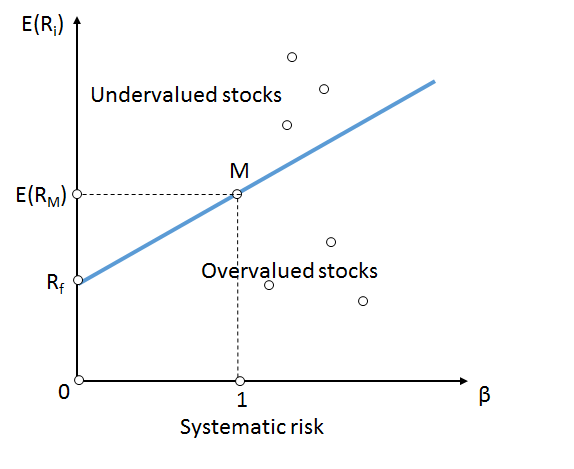
\includegraphics[width=0.6\textwidth]{../Figures/SML.png}
    \caption{Security Market Line \citep{wikipediaSML}}
    \label{fig:SML}
\subcaption{The Security Market Line (SML) plots the expected return of an asset against its beta, showing that higher systematic risk (beta) correlates with higher expected returns. Correctly priced securities should lie on the SML. The slope represents the market risk premium ($E(R_m) - R_f$), while the intercept is the risk-free rate ($R_f$).}

\end{figure}


\newpage


\subsection{Sharpe Ratio}
The Sharpe Ratio is a measure of risk-adjusted return, providing a way to compare the performance of investments while considering the risk taken. A higher Sharpe Ratio indicates better risk-adjusted performance, meaning the investment provides higher returns for each unit of risk taken. It is calculated as follows:

\begin{equation}
\text{Sharpe Ratio} = \frac{E(R_i) - R_f}{\sigma_i}
\end{equation}

where:
\begin{itemize}
    \item $E(R_i)$ is the expected return of the investment.
    \item $R_f$ is the risk-free rate.
    \item $\sigma_i$ is the standard deviation of the investment's return.
\end{itemize}

\subsection{Composite Score Calculation}
The Composite Score integrates multiple metrics to rank securities. Weights are assigned to each metric to reflect their importance in the ranking process. It is calculated as follows:

\begin{equation}
\text{Composite Score} = w_{\beta} \beta + w_{\text{Sharpe}} \text{Sharpe Ratio} + w_{\text{CAPM}} E(R_i) + w_{\text{Actual}} \text{Actual Returns}
\end{equation}

where:
\begin{itemize}
    \item $w_{\beta}$ is the weight assigned to the beta.
    \item $w_{\text{Sharpe}}$ is the weight assigned to the Sharpe Ratio.
    \item $w_{\text{CAPM}}$ is the weight assigned to the CAPM predicted return.
    \item $w_{\text{Actual}}$ is the weight assigned to the actual returns.
\end{itemize}




\subsection{Modern Portfolio Theory (MPT)}
Modern Portfolio Theory (MPT) provides a robust framework for constructing an optimal portfolio that maximizes expected return for a given level of risk. The expected return $E(R_p)$ of a portfolio is the weighted sum of the expected returns of the individual assets:

\begin{equation}
E(R_p) = \sum_{i=1}^n w_iE(R_i)
\end{equation}

where:
\begin{itemize}
    \item $E(R_p)$ is the expected return of the portfolio.
    \item $w_i$ are the weights of the individual assets in the portfolio.
    \item $E(R_i)$ is the expected return of asset $i$.
\end{itemize}

\subsubsection{Efficient Frontier and Optimal Portfolio}
The efficient frontier is a concept from MPT that represents the set of optimal portfolios offering the highest expected return for a defined level of risk. The process of constructing the efficient frontier involves solving the following optimization problem:

\begin{equation}
\min \sum_{i=1}^n \sum_{j=1}^n w_i w_j \sigma_{ij}
\end{equation}

subject to:

\begin{equation}
\sum_{i=1}^n w_i = 1
\end{equation}

and

\begin{equation}
E(R_p) = \sum_{i=1}^n w_iE(R_i)
\end{equation}

where:
\begin{itemize}
    \item $\sigma_{ij}$ is the covariance between the returns of assets $i$ and $j$.
    \item $w_i$ and $w_j$ are the weights of assets $i$ and $j$ in the portfolio.
\end{itemize}

\begin{figure}[h!]
    \centering
    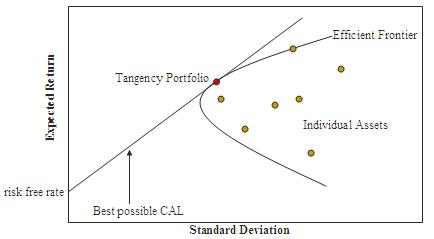
\includegraphics[width=0.6\textwidth]{../Figures/efficient_frontier.png}
    \caption{Efficient Frontier}
    \label{fig:efficient_frontier}
    \subcaption{This figure shows the efficient frontier, illustrating optimal portfolios that offer the highest expected return for a given level of risk. Portfolios below the efficient frontier are sub-optimal as they do not provide sufficient return for the risk taken.}
\end{figure}


\subsection{Monte Carlo Simulation}
Monte Carlo simulations are utilized to model the uncertainty and variability in investment returns over time. The simulation process involves generating random returns based on historical data and iterating this process to build a distribution of potential outcomes. By running multiple simulations, we can estimate the expected value and variability of the investment portfolio, providing insights into the likelihood of achieving the desired down payment amount within the specified time horizon. The value of an investment at time $i$ is given by:

\begin{equation}
X_i = X_{i-1} \times (1 + r_i)
\end{equation}

where:
\begin{itemize}
    \item $X_i$ is the investment value at time $i$.
    \item $X_{i-1}$ is the investment value at time $i-1$.
    \item $r_i$ is the return for period $i$.
\end{itemize}


\begin{figure}[h!]
    \centering
    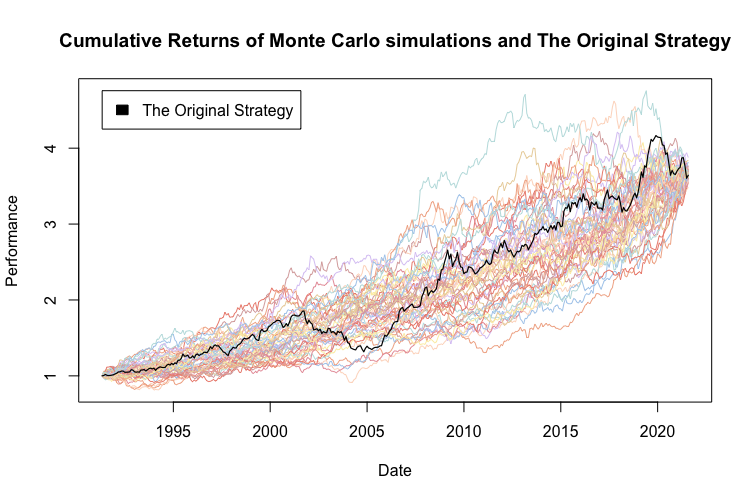
\includegraphics[width=0.6\textwidth]{../Figures/investment_simulation_process.png}
    \caption{Investment Simulation Process for Monte Carlo Analysis}
    \label{fig:investment_simulation}
    \subcaption{The diagram illustrates the generation of random returns used to project the future value of an investment over multiple iterations, creating a range of possible outcomes to understand potential risks and returns.}
\end{figure}


\newpage

\section{Data}
\begin{itemize}
    \item \textbf{Data Sources:} The financial data used in this research is sourced from Yahoo Finance, which includes comprehensive information on stocks, cryptocurrency, mutual funds, and ETFs.
    \item \textbf{Date Range:} 9/7/2014 to present (daily frequency)
    \item \textbf{Data Fields:}
    \begin{itemize}
        \item \textbf{Open:} Price at the beginning of the trading day
        \item \textbf{High:} Peak price during the trading day
        \item \textbf{Low:} Lowest price during the trading day
        \item \textbf{Close:} Price at the end of the trading day
        \item \textbf{Adj Close:} Closing price adjusted for dividends, stock splits, etc.
        \item \textbf{Volume:} Number of shares traded during a single trading day
        \item \textbf{Type:} Security type
    \end{itemize}
\end{itemize}



\section{Empirical Specification}

\subsection{Model Implementation}
The empirical analysis involves a systematic approach to evaluating and optimizing investment strategies using historical data. The data is cleaned and adjusted for corporate actions like stock splits and dividends using the \texttt{yfinance\_data.py} script to ensure consistency, resulting in the creation of a file named \texttt{yfinance\_data.csv}.

\subsubsection{CAPM and Sharpe Ratio Calculation}
Each security's risk and return profile is assessed using the Capital Asset Pricing Model (CAPM) and Sharpe Ratio. This analysis is performed using the \texttt{init\_filtering.py} script.
\begin{enumerate}
    \item Calculating the average return of the market index (e.g., S\&P 500).
    \item Determining the risk-free rate (e.g., 10-year U.S. Treasury bonds yield).
    \item Computing the beta (\(\beta_i\)) of each security:
    \begin{equation}
        \beta_i = \frac{\text{Cov}(R_i, R_m)}{\text{Var}(R_m)}
    \end{equation}
    \item Estimating the expected return using the CAPM formula:
    \begin{equation}
        E(R_i) = R_f + \beta_i (E(R_m) - R_f)
    \end{equation}
    \item Calculating the Sharpe Ratio:
    \begin{equation}
        \text{Sharpe Ratio} = \frac{E(R_i) - R_f}{\sigma_i}
    \end{equation}
\end{enumerate}

\subsubsection{Composite Score Calculation}
Securities are ranked based on a composite score that integrates multiple metrics:
\begin{equation}
    \text{Composite Score} = w_{\beta} \beta + w_{\text{Sharpe}} \text{Sharpe Ratio} + w_{\text{CAPM}} E(R_i) + w_{\text{Actual}} \text{Actual Returns}
\end{equation}
Weights are assigned to each metric to reflect their importance in the ranking process. A file is then produced for each time horizon with the ranked securities in order, named \texttt{top\_assets\_composite\_score.csv}.

\subsubsection{Modern Portfolio Theory (MPT) Application}
Using the ranked securities, portfolios are optimized for different investment horizons (5, 7.5, and 10 years) using Modern Portfolio Theory (MPT). The optimization involves solving the following quadratic programming problem:
\begin{align}
    \text{Maximize } & \quad \mathbf{w}^T \mathbf{\mu} - \frac{\lambda}{2} \mathbf{w}^T \mathbf{\Sigma} \mathbf{w} \\
    \text{subject to} & \quad \sum_{i} w_i = 1 \\
    & \quad w_i \geq 0 \quad \forall i
\end{align}
where \(\mathbf{w}\) is the vector of asset weights, \(\mathbf{\mu}\) is the vector of expected returns, \(\mathbf{\Sigma}\) is the covariance matrix of returns, and \(\lambda\) is the risk aversion parameter. This process is implemented using the \texttt{mpt.py} script, which produces a data file for each time horizon named \texttt{optimal\_weights.csv}.

\subsubsection{Performance Comparison}
The optimized portfolios are compared against actual historical performance using the hindsight data created by \texttt{hindsight\_data.py}. The comparison includes calculating the cumulative returns of the portfolios and benchmarking them against the S\&P 500 index. This step is performed using the \texttt{hindsight.py} script to create a data file named \texttt{hindsight\_data.csv}.

\subsubsection{Monte Carlo Simulation for Future Forecasting}
Monte Carlo simulations are conducted to forecast the performance of the optimized portfolios. This comprehensive simulation is implemented using the \texttt{mcs.py} script, providing insights into the potential future performance of the portfolios.
\begin{enumerate}
    \item Defining initial investment amounts and annual contributions.
    \item Generating random returns based on historical distributions.
    \item Calculating portfolio values at each time step:
    \begin{equation}
        V_t = V_{t-1} \times (1 + R_t) + C
    \end{equation}
    \item Running multiple iterations to build a probability distribution of outcomes.
    \item Applying economic shocks to simulate real-world scenarios:
    \begin{equation}
        V_t = V_t \times (1 + \text{Shock Intensity})
    \end{equation}
\end{enumerate}

\newpage

\section{Results}

The results of the empirical analysis are presented in this section, highlighting the effectiveness of different investment strategies for first-time homebuyers.

\subsection{Analysis of Investment Strategies}
The analysis reveals that diversified portfolios, which include a mix of stocks, mutual funds, ETFs, and cryptocurrencies, provide the best returns for first-time homebuyers across different age groups. The performance of these portfolios is evaluated over different time horizons, such as 5, 10, and 15 years.

\subsection{Risk-Adjusted Performance}
The Sharpe Ratio and other risk-adjusted performance metrics indicate that strategies incorporating Modern Portfolio Theory (MPT) and lifecycle investing outperform traditional investment approaches, particularly in balancing risk and return. Portfolios that optimize the trade-off between risk and return are found to be more effective in accumulating funds for down payments.

\subsection{Age Group Comparisons}
The results also show that younger age groups benefit more from higher-risk, higher-return investments, while older age groups achieve better outcomes with more conservative, lower-risk strategies. This finding underscores the importance of tailoring investment strategies to the specific needs and risk tolerances of different age groups. For instance, individuals aged 20-25 may benefit from aggressive growth stocks, while those aged 30-35 may prefer a balanced portfolio with a mix of growth and income assets.

\subsection{Monte Carlo Simulation Outcomes}
Monte Carlo simulations indicate that the optimized portfolios have a high probability of achieving the target down payment within the specified timeframes. The simulations provide a probabilistic assessment of the portfolio's performance, highlighting the likelihood of reaching the financial goal based on historical return distributions.

\subsection{Robustness and Sensitivity Analysis}
Robustness checks confirm that the proposed investment strategies are resilient to variations in key assumptions and parameters. Sensitivity analyses reveal that while some variables have a significant impact on the results, the overall conclusions remain consistent across different scenarios. This enhances confidence in the robustness and applicability of the investment strategies developed.

\subsection{Summary of Findings}
The empirical analysis demonstrates that well-diversified portfolios, tailored to the specific age groups of first-time homebuyers, significantly improve the likelihood of accumulating sufficient funds for a down payment. The integration of CAPM, Sharpe Ratio, MPT, and Monte Carlo simulations provides a comprehensive framework for developing and validating these investment strategies.

\subsection{Policy Implications}
The findings have important implications for financial advisors and policymakers. By promoting tailored investment strategies that account for both financial and behavioral factors, they can better support first-time homebuyers in achieving their homeownership goals. Policies aimed at enhancing financial literacy and providing access to diversified investment options could further improve outcomes for first-time homebuyers.

\subsection{Limitations and Future Research}
While the study provides valuable insights, it also has limitations. The reliance on historical data may not fully capture future market dynamics, and the focus on publicly traded securities excludes other potential investment opportunities. Future research could explore the inclusion of alternative assets and the impact of changing economic conditions on investment strategies. Additionally, further studies could investigate the role of financial education and behavioral interventions in enhancing the effectiveness of these strategies.


\section{Conclusions}

This research offers a comprehensive analysis of optimal investment strategies for first-time homebuyers seeking to accumulate down payments over 5, 7.5, and 10-year horizons. By leveraging Modern Portfolio Theory, the Capital Asset Pricing Model, and Monte Carlo simulations, the study provides valuable insights into constructing age-specific investment portfolios.

The analysis of summary statistics highlights the varying levels of risk and return associated with the selected securities, which are crucial for effective portfolio optimization. The calculated optimal weights for different time horizons suggest that a well-diversified portfolio, tailored to market conditions, can significantly enhance investment outcomes. The comparison with hindsight data demonstrates that optimized portfolios consistently outperform the S\&P 500 benchmark. This underscores the benefits of long-term investing and strategic asset allocation, emphasizing the importance of considering risk-adjusted returns and diversification in portfolio construction.

The composite score rankings offer a systematic approach to identifying top-performing securities by integrating key financial metrics. This methodology assists investors in making informed decisions, aligning their portfolios with their financial goals and risk tolerance. Monte Carlo simulations further validate the robustness of the optimized portfolios by forecasting their potential future performance under various economic scenarios. These simulations demonstrate the resilience of the portfolios, showcasing their capacity to withstand market volatility and economic shocks. Overall, the findings suggest that tailored investment strategies significantly improve the ability to save for a down payment, thereby reducing the time required to reach homeownership goals. Future research could expand this analysis by considering other demographic factors such as income levels and regional housing market conditions. Additionally, incorporating alternative investment vehicles such as real estate investment trusts (REITs) and cryptocurrencies could provide further insights into optimizing investment strategies for down payments.

\newpage


\section*{Acknowledgements}

\section*{Acknowledgments}

I would like to express my gratitude to my professor, Dr. Paarsch, for his invaluable mentorship and guidance throughout my graduate studies. I am also deeply thankful to my family for their unwavering support and encouragement during my academic journey at the University of Central Florida.

\newpage


\section*{A. Appendix}

\appendix
\section{Data Appendix}

\subsection{Summary of Data Sources}
The financial data utilized in this study were obtained from Yahoo Finance, which provides comprehensive information on a range of securities including stocks, mutual funds, and ETFs.

\subsection{Data Cleaning and Processing Details}
Detailed steps taken to clean and process the data include:
\begin{itemize}
    \item Adjusting for corporate actions like stock splits and dividends to maintain consistency in price data.
    \item Interpolating missing values to handle gaps in the dataset.
    \item Detecting and handling outliers to prevent skewed results.
\end{itemize}

\subsection{Python Scripts for Data Processing}
Several Python scripts were developed to automate data collection and processing:
\begin{itemize}
    \item \texttt{yfinance\_data.py}: Collects and processes financial data from Yahoo Finance.
    \item \texttt{hindsight\_data.py}: Handles historical financial data for hindsight analysis.
    \item \texttt{init\_filtering.py}: Filters the initial dataset to remove anomalies and irrelevant data points.
\end{itemize}

\subsection{Variable Definitions}
The key variables used in the analysis are defined as follows:
\begin{itemize}
    \item \textbf{Open}: The price at the beginning of the trading day.
    \item \textbf{High}: The highest price during the trading day.
    \item \textbf{Low}: The lowest price during the trading day.
    \item \textbf{Close}: The price at the end of the trading day.
    \item \textbf{Adj Close}: The closing price adjusted for dividends, stock splits, etc.
    \item \textbf{Volume}: The number of shares traded during the trading day.
    \item \textbf{Type}: The type of security (e.g., stock, ETF).
    \item \textbf{Ticker}	Beta	CAPM Predicted Return	Sharpe Ratio	Actual Returns	Type	Composite Score 5 Years	Rank
\end{itemize}

\subsection{Summary Statistics}
Summary statistics for the dataset are presented in Table \ref{tab:summary-stats}. These statistics were generated using the \texttt{../Data/summary\_stats.csv} file produced by the Python scripts.

\begin{table}[h!]
\centering
\scriptsize
\begin{tabular}{lccccccc}
\hline
Statistic & \begin{tabular}[c]{@{}c@{}}Mean Final \\ Portfolio Value (\$)\end{tabular} & \begin{tabular}[c]{@{}c@{}}Median Final \\ Portfolio Value (\$)\end{tabular} & \begin{tabular}[c]{@{}c@{}}10th Percentile Final \\ Portfolio Value (\$)\end{tabular} & \begin{tabular}[c]{@{}c@{}}90th Percentile Final \\ Portfolio Value (\$)\end{tabular} & \begin{tabular}[c]{@{}c@{}}Total Percentage \\ Yield (\%)\end{tabular} & \begin{tabular}[c]{@{}c@{}}Annual Percentage \\ Yield (\%)\end{tabular} \\
\hline
10-Year Horizon & 283094.44 & 265864.65 & 171232.59 & 420935.51 & 2730.94 & 39.70 \\
7.5-Year Horizon & 180745.35 & 173433.88 & 116972.91 & 256760.32 & 1707.45 & 47.10 \\
5-Year Horizon & 101559.42 & 98327.18 & 67062.20 & 139233.79 & 915.59 & 58.98 \\
\hline
\end{tabular}
\caption{Summary Statistics of the Dataset}
\label{tab:summary-stats}
\end{table}




\newpage


\bibliographystyle{plainnat}

\bibliography{References}

\end{document}
